\documentclass[./exercises.tex]{subfiles}
\begin{document}
\textit{\textbf{Tentamen 2021-08-18 } }\\

\begin{enumerate}
\item  Du ska blanda till 5 liter vatten som ska ha temperaturen 40°C genom blandning
     av två vattenmängder: en med 10°C och en med 90°C. Hur stora är dessa mängder?\\

Givet 
\begin{flalign*}
V_{tot} &= 5 \text{ liter}\\
T_1 &= 10^o\text{C}\\
T_2 &= 90^o\text{C}\\
T_f &= 40^o\text{C}\\
\end{flalign*}
Mass balansen
\begin{flalign*}
m_1+m_2 &=m_{tot}\\
\rho\cdot V_1+\rho \cdot V_2 &= \rho\cdot V_{tot}\\
\end{flalign*}
Energi balans är
\begin{flalign*}
|Q_{avgiven}|&=|Q_{upptagen}|\\
m_2\cdot c\cdot(90-40)&=m_1\cdot c\cdot(40-10)\\
\end{flalign*}
Ersätt en av variablerna $m_2$ eller $m_1$ med
sambandet från mass-balansen.
\begin{flalign*}
(m_{tot}-m_1)\cdot c\cdot 50 &=m_1\cdot c\cdot30\\
\end{flalign*}
Lös ut $m_1$
\begin{flalign*}
m_{tot}\cdot c\cdot 50 &=m_1\cdot c\cdot30+m_1\cdot c\cdot50\\
                  &=m_1\cdot(30+50)\cdot c\iff\\
m_1 &=\frac{50}{80}\cdot m_{tot}
\end{flalign*}
Således skall blandningen vara $5/8$ delar kallt vatten
och $3/8$ delar varmt vatten
Eller explict uträknat
\begin{flalign*}
V_1 &=\frac{5}{8}\cdot 5 = \frac{25}{8} = 3.125 \text{ liter 10 gradigt}\\
V_2 &= 5-3.125 =1.875 \text{ liter 90 gradigt}\\
\end{flalign*}

\vfill\null
\clearpage
\columnbreak
\newpage

\item En behållare har volymen 15.0 l och innehåller 0.010 kg syrgas\\\
($\kappa =1.40$    $R = 260$ J/ kg *K, som har temperaturen $+27^o$ C.
Gasen får expandera adiabatiskt till slutvolymen 45.0 l .\\
Vilket tryck får gasen. Rita processen i ett p/V-diagram och i ett T/S-diagram.\\

Givet
\begin{flalign*}
V_1 &= 15\text{ liter} = 0.015\text{ m}^3\\
T_1 &= +27^o\text{C}= 300^o\text{K}\\
m &=0.010 \text{ kg}\\
V_2 &= 45\text{ liter} = 0.045\text{ m}^3\\ 
\kappa &= 1.4\\
R &= 260\text{ J/kg*K}\\
\end{flalign*}
Allmänna gaslagen ger trycket $p_1$
\begin{flalign*}
p_1\cdot V_1 &=m\cdot R\cdot T_1\\
p_1 &=\frac{m\cdot R\cdot T_1}{V_1}\\
    &=\frac{0.01\cdot 260\cdot 300}{0.015}\\
    &=52000\text{ Pa}
\end{flalign*}
Den adiabatiska expansionen förhåller sig enligt
\begin{flalign*}
p_1\cdot V_1^\kappa &=p_2\cdot V_2^\kappa\\
p_2 &= p_1\cdot \Big(\frac{V_1}{V_2}\Big)^\kappa\\
    &= 52000\cdot \Big(\frac{0.015}{0.045}\Big)^{1.4}\\
    &=11169.4962\text{ Pa}\approx 11169.5 \text{ Pa}\\
\end{flalign*}
Den jäklen vill att man ska svara med två värde siffror
alltså $11$kPa.\\

\vfill\null
\clearpage
\columnbreak
\newpage

\item En cylinder med volymen $0.005 m^3$ innehåller helium ($\kappa = 1.67$) 
med trycket 200 kPa och temperaturen $25^o$C. Rita processen i ett p/V-diagram.
Beräkna den värmemängd som måste överföras för att åstadkomma en isoterm expansion
till dubbla volymen. Ska värmemängden bortföras eller tillföras?\\

Givet:\\
\begin{flalign*}
p_1 &=200\cdot 10^3 \text{ Pa}\\
V_1 &= 0.005\text{ m}^3\\
T &=25^o\text{C} = 298^o\text{K}\\
\end{flalign*}
Formeln för $Q$ i en isoterm process innehåller $m\cdot R\cdot T$ vilken vi kan ta fram genom 
allmänna gaslagen
\begin{flalign*}
m\cdot R\cdot T&=p_1\cdot V_1\\
               &=200\cdot 10^3\cdot 0.005\\
\end{flalign*}
Formeln kan tas fram
\begin{flalign*}
dQ &= dU+p\cdot dV\\
\end{flalign*}
$dU$ är noll för en isoterm process
\begin{flalign*}
dQ &= p\cdot dV\\
\int_1^2 dQ &= \int_1^2 p\cdot dV\\
Q_{12}       &=\int_1^2 \frac{m\cdot R\cdot T}{V}dV
             &=m\cdot R\cdot T ln\Big(\frac{V_2}{V_1}\Big)
\end{flalign*}
Nu kan $Q_{12}$ beräknas
\begin{flalign*}
Q_{12}&=m\cdot R \cdot T\cdot ln\Big(\frac{V_2}{V_2}\Big)\\
  &=m\cdot R \cdot T\cdot ln\Big(\frac{2V_1}{V_1}\Big)\\
  &=200\cdot 10^3\cdot 0.005 ln(2)\\
  &=693.14718056 \text{J}
\end{flalign*}
Svar med två värdesiffror blir 0.69kJ.\\

\vfill\null
\clearpage
\columnbreak
\newpage

\item  I en kompressor som suger in $12.0 \text{m}^3$ luft per minut går luften
ifrån $1.05$ bar och 300 K till $12.0$ bar och 400 K.
Vid kompressionen bortförs $2.00$ kW värme.
Beräkna vilken tillförd effekt kompressorn kräver.
Är processen isoterm, adiabatisk eller en polytrop?\\
( $\kappa$ = 1.40     $c_p$ = 1.006 kJ/kg      $\rho$ = 1.20 kg/m3)\\

Givet:\\
\begin{flalign*}
\dot{V}&=12/60 \text{m}^3/\text{s}=0.2\text{m}^3/\text{s}\\
p_1 &= 1.05\cdot 10^5 \text{Pa}\\
T_1 &= 300^o\text{K}\\
p_2 &= 12\cdot 10^5 \text{Pa}\\
T_2 &= 400^o\text{K}\\
\dot{Q}_{12} &= -2000\text{W}\\
\end{flalign*}
Adiabatisk är den inte eftersom värme bortförs. Vi avgör om processen
är isoterm eller polytrop genom att identifiera om
koefficienten $n \neq 1$
För en polytrop process gäller 
\begin{flalign*}
\frac{T_2}{T_1}&=\Big(\frac{p_2}{p_1}\Big)^{\frac{n-1}{n}}\\
ln \frac{T_2}{T_1}&=\frac{n-1}{n}\cdot ln\Big(\frac{p_2}{p_1}\Big)\iff\\
\frac{n-1}{n} &= ln \frac{T_2}{T_1}/ln\frac{p_2}{p_1}\\
n-1 &=n\cdot ln \frac{T_2}{T_1}/ln\frac{p_2}{p_1}\\
\end{flalign*}
Samlar ihop lika termer
\begin{flalign*}
n&(1-ln \frac{T_2}{T_1}/ln\frac{p_2}{p_1})=1\\
n&=\frac{1}{(1-ln \frac{T_2}{T_1}/ln\frac{p_2}{p_1})}\\
 &=\frac{1}{(1-ln \frac{400}{300}/ln\frac{12}{1.05})}\\
 &=1.133903121
\end{flalign*}
Således polytrop.\\

Formeln för ett öppet system är
\begin{flalign*}
\dot{Q}_{12} &= \dot{I_2}-\dot{I_1} + \dot{W}_{t2}\\
\end{flalign*}
Löser ut $\dot{W}_{t2}$\\
\begin{flalign*}
\dot{W}_{t2}&=\dot{Q}_{12} -( \dot{I_2}-\dot{I_1})\\
            &=\dot{Q}_{12} -\dot{m}\cdot\bar{c}_p\cdot(T_2-T_1)\\
             &=\dot{Q}_{12} -\rho\dot{V}\cdot\bar{c}_p\cdot(T_2-T_1)\\
			 &=-2000 - 1.20\cdot 0.2\cdot 1006\cdot(400-300)\\
			 &=-26144\text{W}
\end{flalign*}
Kompressorn kräver effekten 26.1kW

\vfill\null
\clearpage
\columnbreak
\newpage

\item Visa, genom att beräkna entropiändringarna för delprocesserna i figuren nedan,
  att totala entropiändringen för gasen är noll. Processen 1 till 2, är en isoterm.

\begin{figure}[H]
  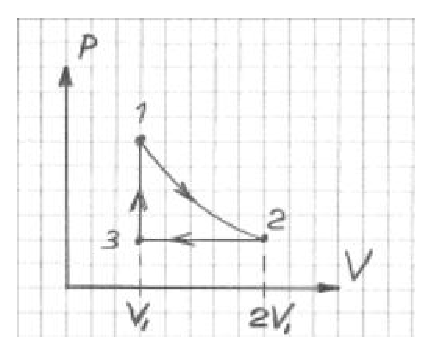
\includegraphics[width=\linewidth]{process.eps}
  \caption{Hypotetisk process}
  \label{fig4}
\end{figure}

Processen som går från $1$ till $2$ är en isoterm till dubbla volymen
\begin{flalign*}
s_2-s_1 &= R\cdot ln \frac{V_2}{V_1}\\
        &= R\cdot ln 2\\
\end{flalign*}
och eftersom $p_1\cdot V_1 = p_2\cdot V_2$
så är $p_2 = p_1/2$
Processen $2$ till $3$ är en isobar som går från volymen $2V_1$ till $V_1$.
\begin{flalign*}
s_3-s_2 &=\bar{c}_p\cdot ln \frac{V_3}{V_2}\\
        &=\bar{c}_p \cdot ln \frac{V_1}{2V_1}\\
        &=-\bar{c}_p\cdot ln 2\\
\end{flalign*}

Processen $3$ till $4$ är en isokor där trycket går från $p_1/2$ till $p_1$
\begin{flalign*}
s_4-s_3 &=\bar{c}_v\cdot ln \frac{p_4}{p_3}\\
        &=\bar{c}_v\cdot ln \frac{p_1}{p_1/2}\\
       &=\bar{c}_v\cdot ln 2\\
\end{flalign*}


Summerar entropiändringarna
\begin{flalign*}
&R\cdot ln 2-\bar{c}_p\cdot ln 2+\bar{c}_v\cdot ln 2\\
&=R\cdot ln 2-(\bar{c}_p-\bar{c}_v)\cdot ln 2\\
&=0
\end{flalign*}

\vfill\null
\clearpage
\columnbreak
\newpage

\item En carnotmaskin arbetar kontinuerligt mellan $350^o$C och $50^o$C.
Maskinen roterar med 800 varv per minut. Vilket spillvärmeflöde måste maskinen
kunna göra sig av med om den ska leverera en mekanisk effekt på 150 kW.\\

Givet:
\begin{flalign*}
T_1 &= 50^o\text{C} =323^o\text{K}\\
T_1 &= 350^o\text{C} =623^o\text{K}
\dot{W}_t &=150\text{ kW}
\end{flalign*}
Sökt är $\dot{Q}_{bortf}$

Carnotmaskinens verkningsgrad är
\begin{flalign*}
\eta_c &= 1- \frac{T_1}{T_2}(1)\\
       &=1- \frac{323}{623}\\
       &=0.481540931
\end{flalign*}
Den generella formeln för verkningsgrad som gäller
oavsett maskintyp är
\begin{flalign*}
\eta &= \frac{W_t}{Q_{tillf}}&(2)\\
\end{flalign*}
Denna kvot är härledd för ett varv i process cykeln men måste också
gälla för 800 varv samt 800 varv dividerat med gemensamfaktor (per tidsenhet)
så vi tar resultatet av $\eta_c$ från ekvation $1$ och sätter in det
i vänsterledet av $2$.
\begin{flalign*}
\eta &= \frac{\dot{W}_t}{\dot{Q}_{tillf}}&(2)\\
0.481540931&=\frac{150 000}{\dot{Q}_{tillf}}\iff\\
\dot{Q}_{tillf}&=\frac{150 000}{0.481540931}\\
         &=311499.999986502
\end{flalign*}
Men
\begin{flalign*}
\dot{Q}_{tillf}&-\dot{Q}_{bortf}=\dot{W}_t\iff\\
\dot{Q}_{bortf}&= \dot{Q}_{tillf}-\dot{W}_t\\
               &=311499.99-150 000\\
			   &=161499.999986502\approx 161500
\end{flalign*}
Svar med tre värdesiffror 161kW måste bortföras.

\vfill\null
\clearpage
\columnbreak
\newpage

\item Torr mättad vattenånga med trycket $20$ bar expanderar
     adiabatiskt ner till $5.0$ bar då den passerar en turbin.
     Beräkna ångans entalpiändring.\\
	 
Detta är en öppen process.

Om ångan är torr mättad så är $x=1$
och entalpin $i''=2798.96$ kJ per kg torrluft. Om den expanderar till
ett lägre tryck så förblir ångan torr mättad eller så blir den
överhettad tror jag. Chansar på att den fortfarande är torr mättad
$i''(5bar) = 2748.79$
\begin{flalign*}
\Delta i &=i''(20)-i''(5)\\
         &=2798.96-2748.79\\
		 &=50.17 \text{ kJ per kg torrluft}
\end{flalign*}

NEEEEEEEEEEEEEEEJ! Detta är fel! Adiabatisk expansion
menas att $s_2 = s_1$!!!

\begin{flalign*}
s_1(20) &=s''(20) = 6.3403 \text{ kJ per Kevin och kg torrluft}
\end{flalign*}
Adiabatisk expansion betyder att $s_{efter} = s_{före}$ eller som i detta fallet $s_2(5) = s_1(20)$.
Nu kan $x_2$ den specifika ånghalten beräknas.
\begin{flalign*}
s_1(20) &= s_2(5)= (1-x_2)\cdot s_2' +x_2\cdot s_2''\\
      s_2-s_2'  &=(s_2''-s_2')\cdot x_2\iff\\
	  x_2 &=\frac{s_2-s_2'}{s_2''-s_2'}\\
	      &=\frac{6.3403-1.8604}{6.8219-1.8604}\\
          &=0.902932581
\end{flalign*}

Entalpin efter expansionen till $5$ bar blir därför
\begin{flalign*}
i_2 &= (1-x_2)\cdot i_2'+ x_2\cdot i_2''\\
    &=(1-x_2)\cdot 640.16+ x_2\cdot 2748.79\\
    &=2544.110728274
\end{flalign*}
Skillnaden i entlapin blir
\begin{flalign*}
\Delta i_{12} &=i_2-i_1\\
        &=2544.110728274-2798.96\\
        &=-254.849271726 \text{ kJ per kg torrluft}\\
\end{flalign*}
Svar med två värdesiffror är
att ändringen i entalpi är -0.25 MJ per kg torrluft.

Här ska man också skissera ångan entalpi-ändring i ett $T-s$-diagram för
fuktig ånga där utgångsläget $1$ måste ligga på linjen som är den högra delen av ``berget''.

\hspace{0.5em}   ----\\
\hspace{3em}    / \hspace{1em}     $\backslash$ $p_1$\\
\hspace{2em} / \hspace{1.5em}    $|\backslash p_2$\\
\hspace{1em}  /  \hspace{2em}        $\backslash$\\

\vfill\null
\clearpage
\columnbreak
\newpage

\item För en luftmängd har man mätt den torra temperaturen till $+25^o$C.
och den våta temperaturen till $+15^o$C.
Bestäm luftens RH, x och i (specifik entalpi).
Till vilken temperatur kan man kyla innan dimma börjar att bildas?
Ta data ifrån bifogat Mollier-diagram.
Rita en förenklad skiss över Mollier-diagrammet där du markerar
alla intressanta tillstånd och de värden du avläser i det bifogade Mollier-diagrammet.
Lämna in din skiss tillsammans med dina lösningar.

\begin{figure}[H]
  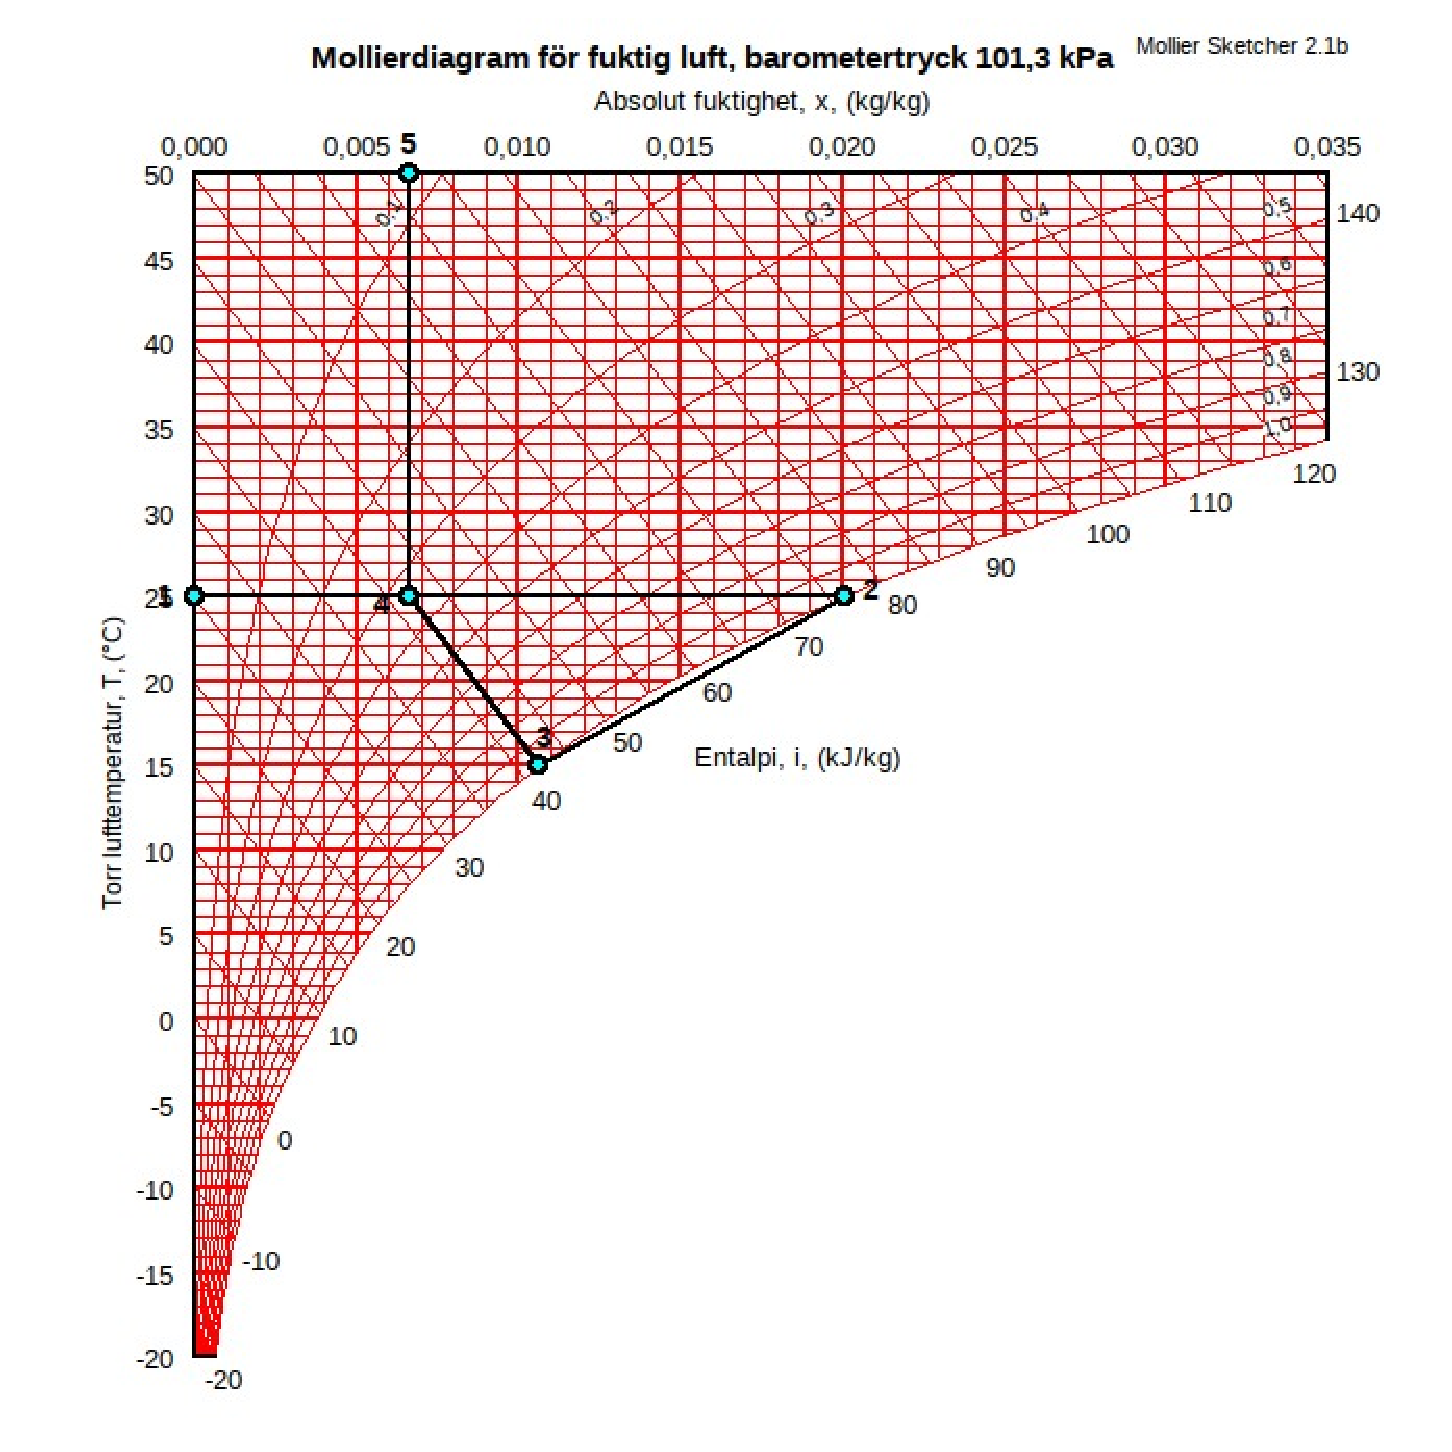
\includegraphics[width=\linewidth]{process2.eps}
  \caption{Mollier diagram}
  \label{fig4}
\end{figure}

Specfika luftfuktigheten/Luftens relativa ångtryck $\varphi = 0.33$, Entalpin
är $42$ kJ per kg torrluft. Ångkvoten $x$ är ca 6.7 gram vatten per kg torrluft
och man kan kyla till $+15^o$C innan dimbildning. \textbf{Fel!} Kylning av luft innebär att
$x=$ konstant.

\begin{figure}[H]
  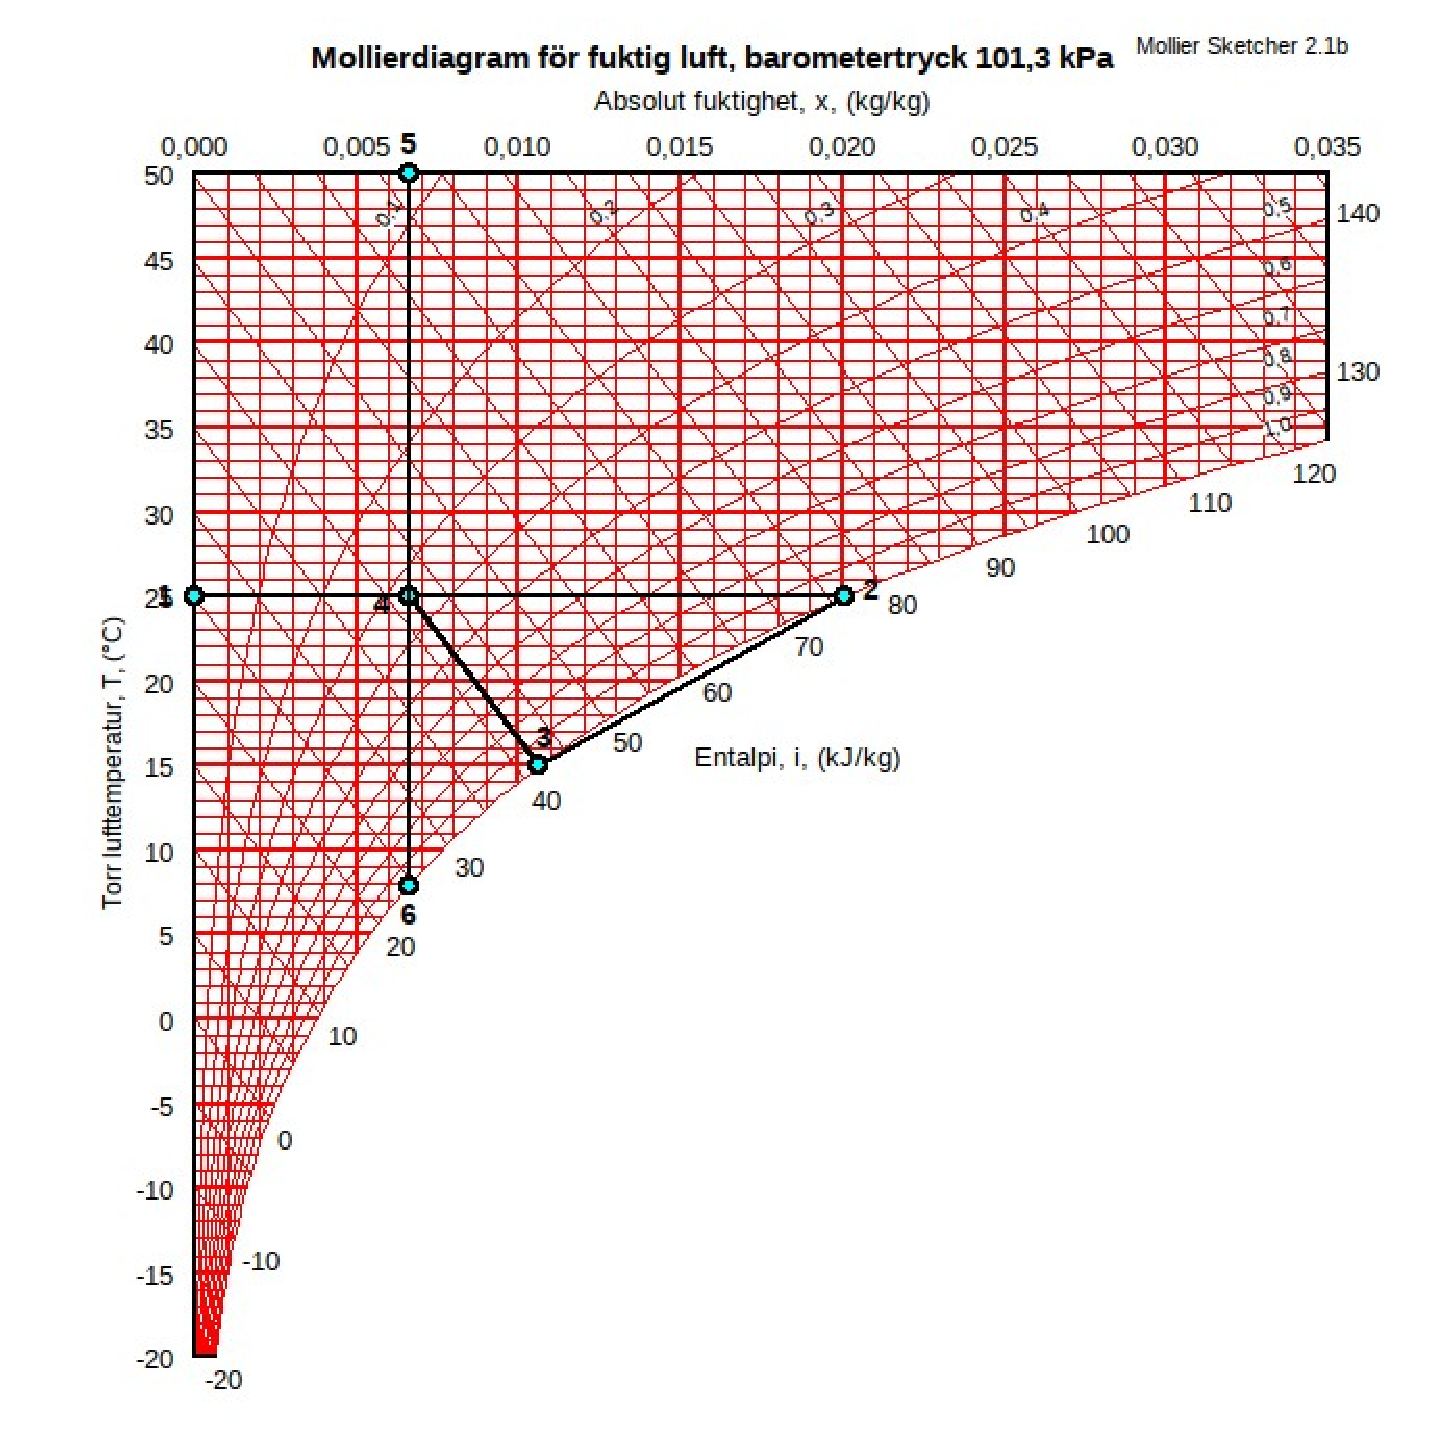
\includegraphics[width=\linewidth]{process3.eps}
  \caption{Mollier diagram 2}
  \label{fig4}
\end{figure}

Följer man konstant $x-$linjen ner till luftfuktighet $100\%$ så fås temperature
$+8^o$C som gränstemperatur för dimbildning.

\end{enumerate}

%\underbrace{}

% \hspace{1em}

%\begin{enumerate}[label=(\alph*)]
%\end{enumerate}


%\vfill\null
%\clearpage
%\columnbreak
%\newpage

%$$
%  A = 
%  \begin{bmatrix}
%    1 & 0  & 2i\\
%    2i & 0 &  -4\\
%    -i &  0 & -2i\\
%  \end{bmatrix}
%$$

%\begin{flalign*}
%  A = 
%  \begin{bmatrix}
%    1 & 0  & 2i\\
%    2i & 0 &  -4\\
%    -i &  0 & -2i\\
%  \end{bmatrix}
%\end{flalign*}


%\begin{flalign*}
%\psi(x) = \begin{cases} Ae^{ikx}+Be^{-ikx} &\ \  x<-a \\
%                        Ce^{\kappa x}+De^{-\kappa x} &\ \ -a < x < a\\
%						Fe^{ikx} & \ \ x>a
%       \end{cases}
%\end{flalign*}

%\begin{figure}[H]
%  \includegraphics[width=\linewidth]{odd_finite.eps}
%  \caption{$z_0=0.1\pi,0.5\pi, 3\pi,7\pi$}
%  \label{fig4}
%\end{figure}
\end{document}
